\section{Performance}
\subsection{Microbenchmarks}

A selection of tailored micro-benchmarks were created to investigate the effects of the transformation on individual parts of code.

\subsubsection{Safe Pointer Dereference}

\begin{verbatim}
// Setup
int x;
int y=malloc(sizeof(int));
// Benchmarked Code
x=*y;
\end{verbatim}

As \verb!y! is recognised as a safe pointer, no bounds checking will be carried out, however at the moment the variable is not marked as \verb!not-NULL!, therefore a null check is performed.
This null check incurs an overhead of \verb!4.6%!.

If there null check were omitted, the only overhead of the fat pointer approach would be the load required to retrieve the fat pointer value.
This benchmark was run without the null check, and the load was found to incur an overhead of \verb!0.9%!.

\subsubsection{Unsafe Pointer Dereference}

\begin{verbatim}
// Setup
int x;
int y=malloc(sizeof(int));
x=y[0];
// Benchmark Code
x=*y;
\end{verbatim}

By using array addressing on the pointer, the CCured analysis detects \verb!y! as a pointer that has arithmetic done on it, and is therefore not \textit{SAFE}.
Therefore the pointer dereference will contain the full bounds check, which was found to incur an overhead of \verb!52%!.

The bounds check function used was complex, first it checked if the value was null, then if the base was null (signifying a pointer of type \verb!NoBounds!), and finally if the value were within the base and bound.
This could be simplified.

\subsubsection{Pointer Allocation}

\begin{verbatim}
// Setup
void Fun1(){}
void Fun2(){int *a,*b,...,*j;}
\end{verbatim}

Many calls were made to \verb!Fun1! and to \verb!Fun2! and the difference in execution time was measured.
This benchmark needed to be done this way because memory used by an allocation is not free until the scope it is allocated in is left, therefore if the allocation were performed in a loop, the stack would run out of space.

This was found to produce no measurable difference.

\subsubsection{Pointer Assignment}

\begin{verbatim}
// Setup
int *a,*b;
// Benchmark Code
a=b;
\end{verbatim}

There is no bounds checking on this code as no pointers are dereferenced, its purpose is to observe the overhead of copying three pointers instead of one.

This was found to produce no measurable difference.

\subsubsection{Cache Contention}

Since fat pointers are three times as large as raw pointers, they cause increased cache usage.
For this benchmark, bounds checks were disabled.

\textbf{Unfortunately, on zenith this wasn't found to produce any performance difference.}

\subsubsection{Following a Linked List}

This benchmark was created to highlight the difference between the fat pointer and the lookup table approach, since with SoftBound no table lookup occurs for local variables.
A linked chain is created and then followed.

\textbf{Initial Results Here}

These tests were repeated with a linked lists of different lengths to investigate how each approach scales with the number of pointers that it needs to keep track of.

\begin{figure}
\centering
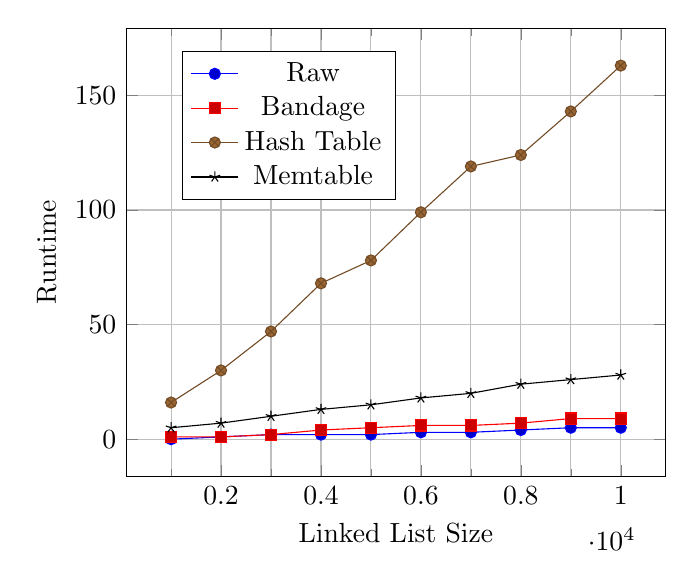
\begin{tikzpicture}
  \begin{axis}[ 
      xlabel=Linked List Size,
      ylabel=Runtime,
      minor x tick num=1,
      grid=both,
	  legend style={at={(0.5,0.95)}}
    ] 
    \addplot coordinates{
		(	1000	,	0	)
		(	2000	,	1	)
		(	3000	,	2	)
		(	4000	,	2	)
		(	5000	,	2	)
		(	6000	,	3	)
		(	7000	,	3	)
		(	8000	,	4	)
		(	9000	,	5	)
		(	10000	,	5	)
    }; 
	\addlegendentry{Raw}
    \addplot coordinates{
		(	1000	,	1	)
		(	2000	,	1	)
		(	3000	,	2	)
		(	4000	,	4	)
		(	5000	,	5	)
		(	6000	,	6	)
		(	7000	,	6	)
		(	8000	,	7	)
		(	9000	,	9	)
		(	10000	,	9	)
    }; 
	\addlegendentry{Bandage}
    \addplot coordinates{
		(	1000	,	16	)
		(	2000	,	30	)
		(	3000	,	47	)
		(	4000	,	68	)
		(	5000	,	78	)
		(	6000	,	99	)
		(	7000	,	119	)
		(	8000	,	124	)
		(	9000	,	143	)
		(	10000	,	163	)
	}; 
	\addlegendentry{Hash Table}
    \addplot coordinates{
		(	1000	,	5	)
		(	2000	,	7	)
		(	3000	,	10	)
		(	4000	,	13	)
		(	5000	,	15	)
		(	6000	,	18	)
		(	7000	,	20	)
		(	8000	,	24	)
		(	9000	,	26	)
		(	10000	,	28	)
	}; 
	\addlegendentry{Memtable}
  \end{axis}
\end{tikzpicture}
\caption{Increase in runtime following a Linked List as size increases}
\label{fig:LinkedListScaling}
\end{figure}


\section{Olden Benchmarks}

\subsection{Treeadd}

The treeadd benchmark constructs a binary tree where each node contains a value in addition to two children (all values are set to 1).
A depth-first search is then performed, accumulating the value at each node.

The implementation of CCured-like analysis counts all member pointers as a non-SAFE type (since the actions on the pointer and therefore the CCured type will be different for each instance), meaning that the tree traversal doesn't benefit from CCured-analysis.

Under Bandage, the tree construction stage, dominated by memory allocations took a \verb!42%! performance hit and the tree traversal stage took a \verb!77%! performance hit.

% 744809 223446 968255
% 1060893 395186 1456079
% Unoptimized bounds checking

\subsection{Bisort}

\section{Correctness}



%\section{Misc}
%\subsection{Fat Pointers}

%Fat pointers add a storage overhead in the pointer itself, tripling its size to that of three pointers.
%Fat pointers generate computational overhead on creation, where the base and bound must be set as well as the value and on dereference, where an extra load instruction must be added.
%Finally fat pointers create computational overhead on bounds checking.

%\subsection{Fat Pointers with CCured Analysis}

%\subsubsection{Safe pointers as Raw or Fat Pointers}

%When combining the CCured approach with the fat pointer analysis, there is a choice of how to implement pointers designated as SAFE - these are pointers that do not require bounds checks on dereference.
%These SAFE pointers can either be implemented as a fat pointer but without bounds checking or kept as a raw pointer.

%Implementing SAFE pointers as fat pointers but without the bounds checking brings consistency but keeps the overhead of fat pointers, which isn't used when SAFE pointers are kept as raw pointers.
